\begin{frame}
  \frametitle{Breast cancer data: application}

  Two cohorts with both proteomic and transcriptomic data
  \begin{enumerate}
    \item \emphase{NCI-60}: $n=60$ diverse human cancer cell lines, $p=91$
    \item  \emphase{RATHER}: $n=100$ sample from patients with breast cancer, $p=117$
  \end{enumerate}

\begin{figure}[htbp!]
  \centering
  \begin{tabular}{@{}cc@{}}
   RATHER & NCI-60 \\
    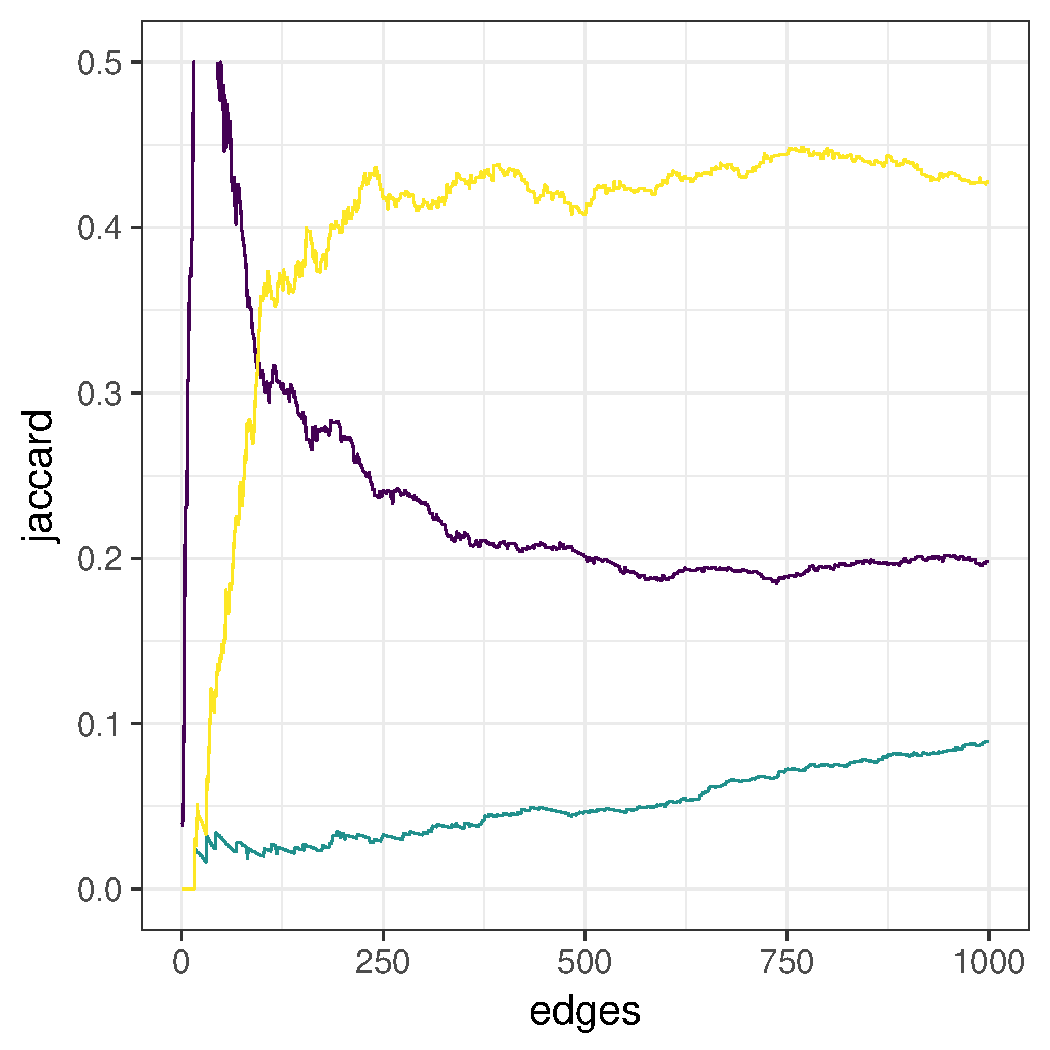
\includegraphics[width=.35\textwidth]{../../chapter/figures/jaccard_RATHER}
  & 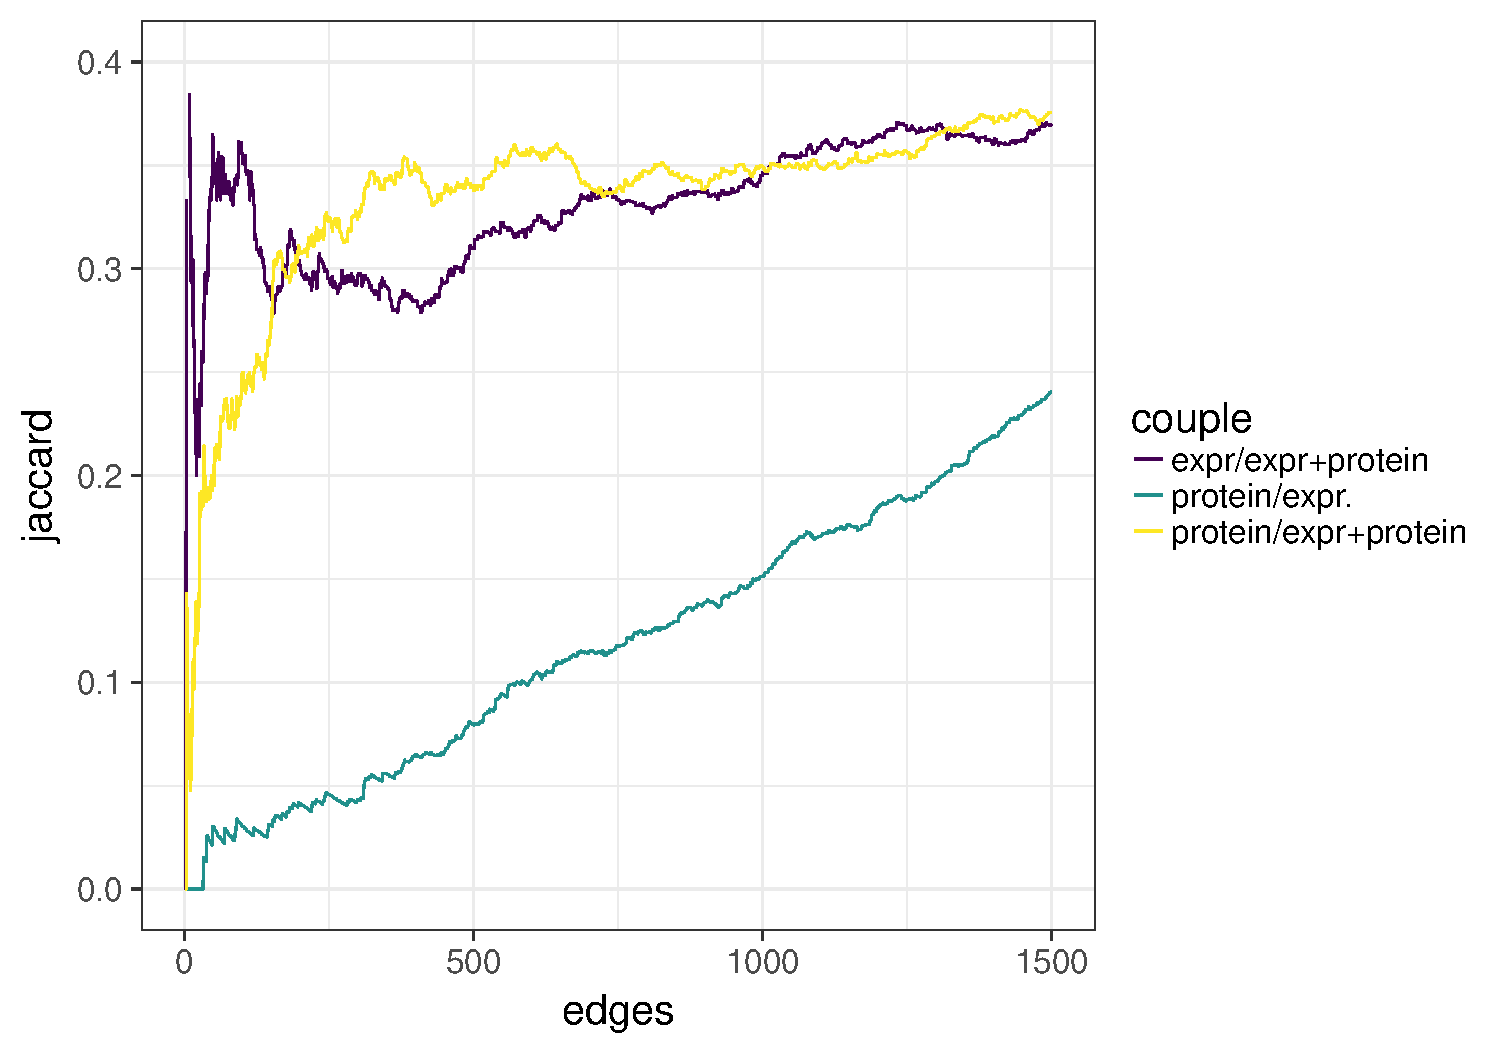
\includegraphics[width=.5\textwidth]{../../chapter/figures/jaccard_NCI60}
  \end{tabular}
  \caption{Jaccard's similarity index
    $J(A,B) = \frac{\left|A\cap B\right|}{\left|A\cup B\right|}$
    between uni-attribute and multiattribute networks, for RATHER and
    NCI60 data set: multiattribute networks share a high Jaccard
    index with both uni-attribute networks.}
  \label{fig:jaccard}
\end{figure}

\end{frame}

\begin{frame}
  \frametitle{Inferred networks}
  
\begin{figure}[htbp!]
  \centering
  \begin{tabular}{@{}lccc@{}}
    & proteomic network  & transcriptomic network  & multiattribute network \\
    \rotatebox{90}{\hspace{1.2cm}NCI60} 
    & 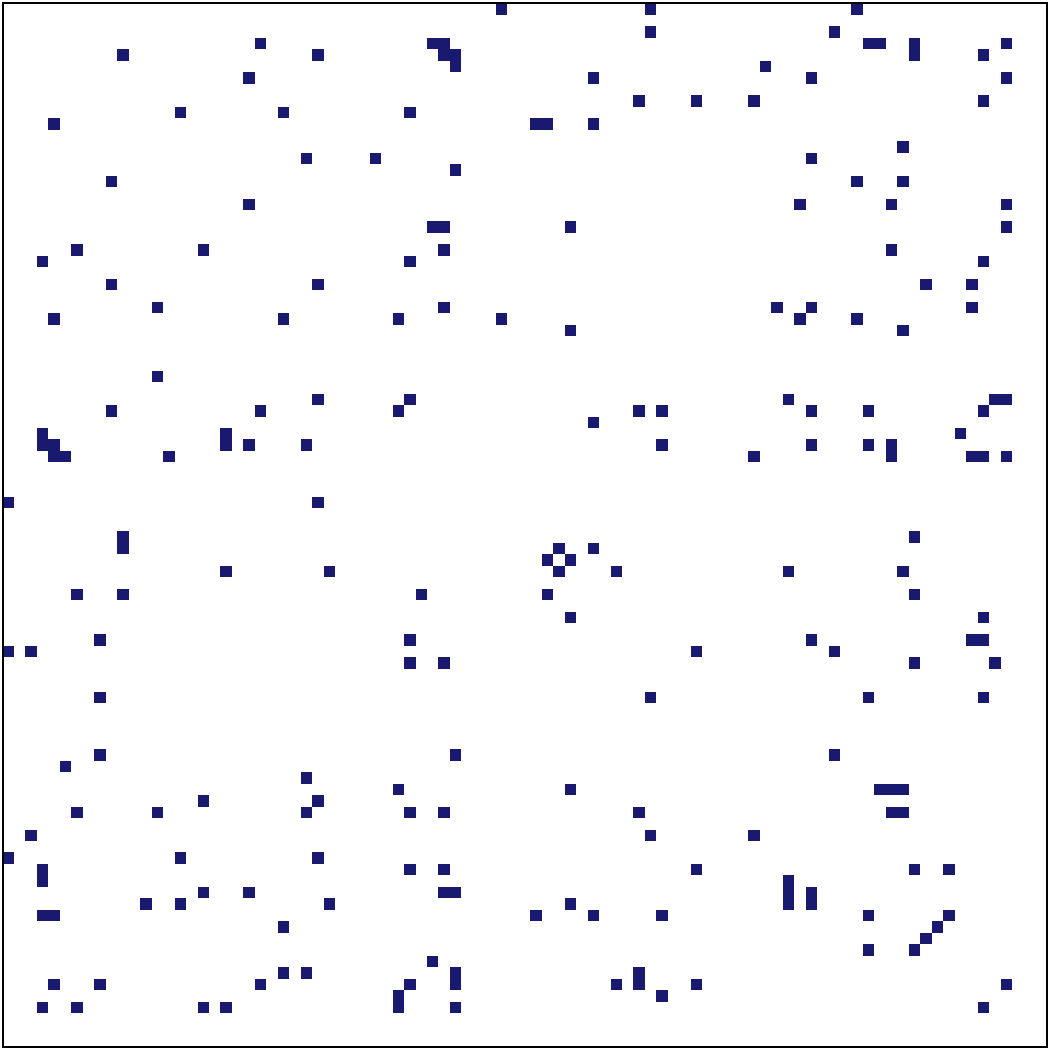
\includegraphics[width=.25\textwidth]{../../chapter/figures/protNet_NCI60}
    & 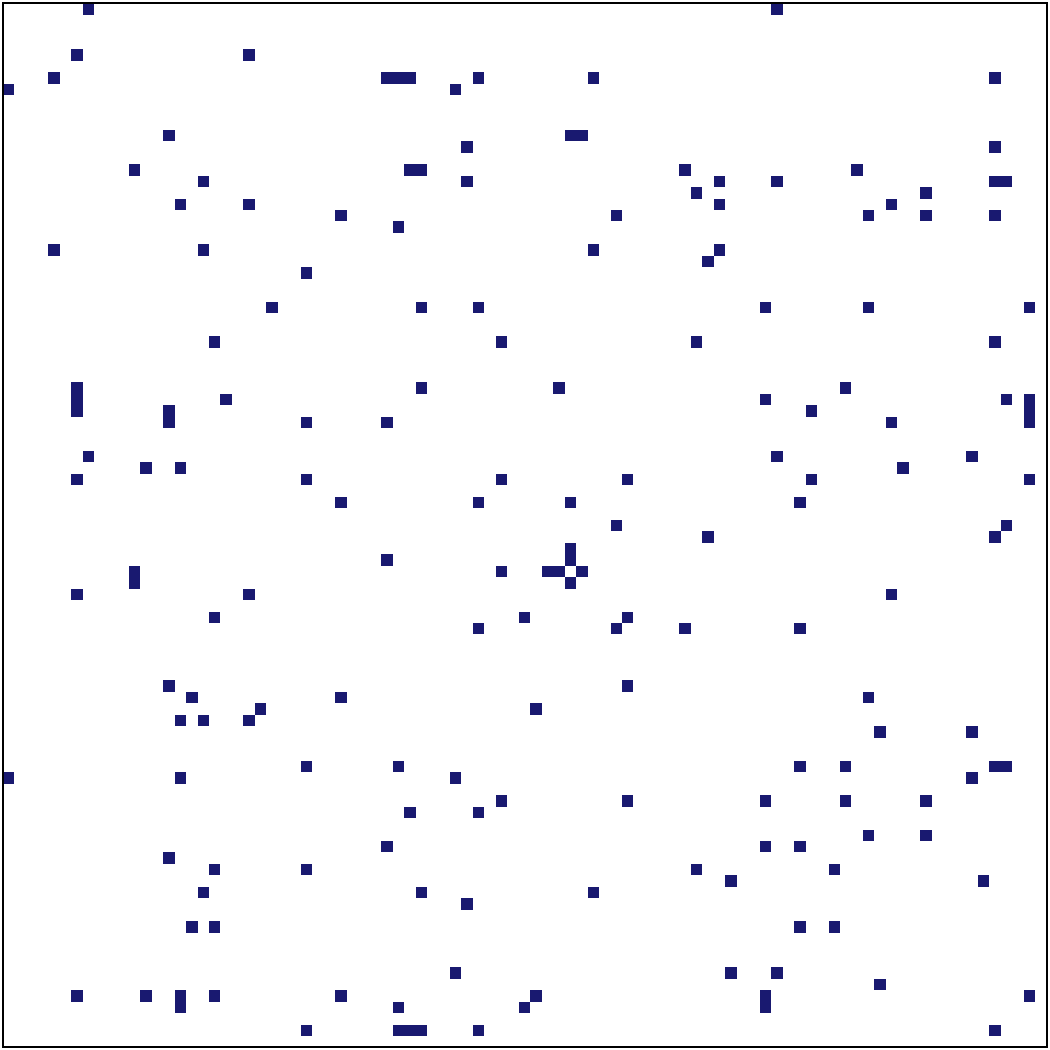
\includegraphics[width=.25\textwidth]{../../chapter/figures/exprNet_NCI60}
    & 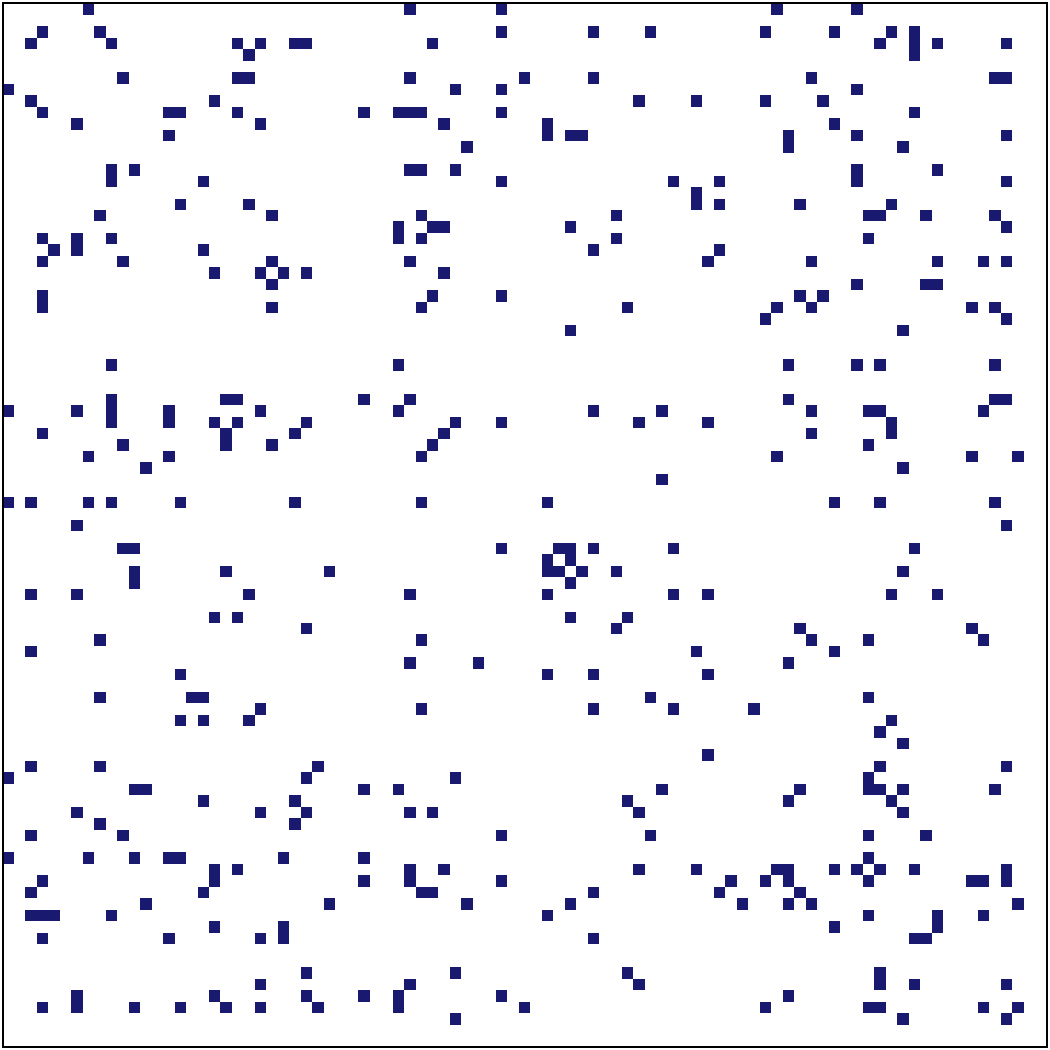
\includegraphics[width=.25\textwidth]{../../chapter/figures/bivarNet_NCI60} \\
    \rotatebox{90}{\hspace{1.2cm}RATHER} 
    & 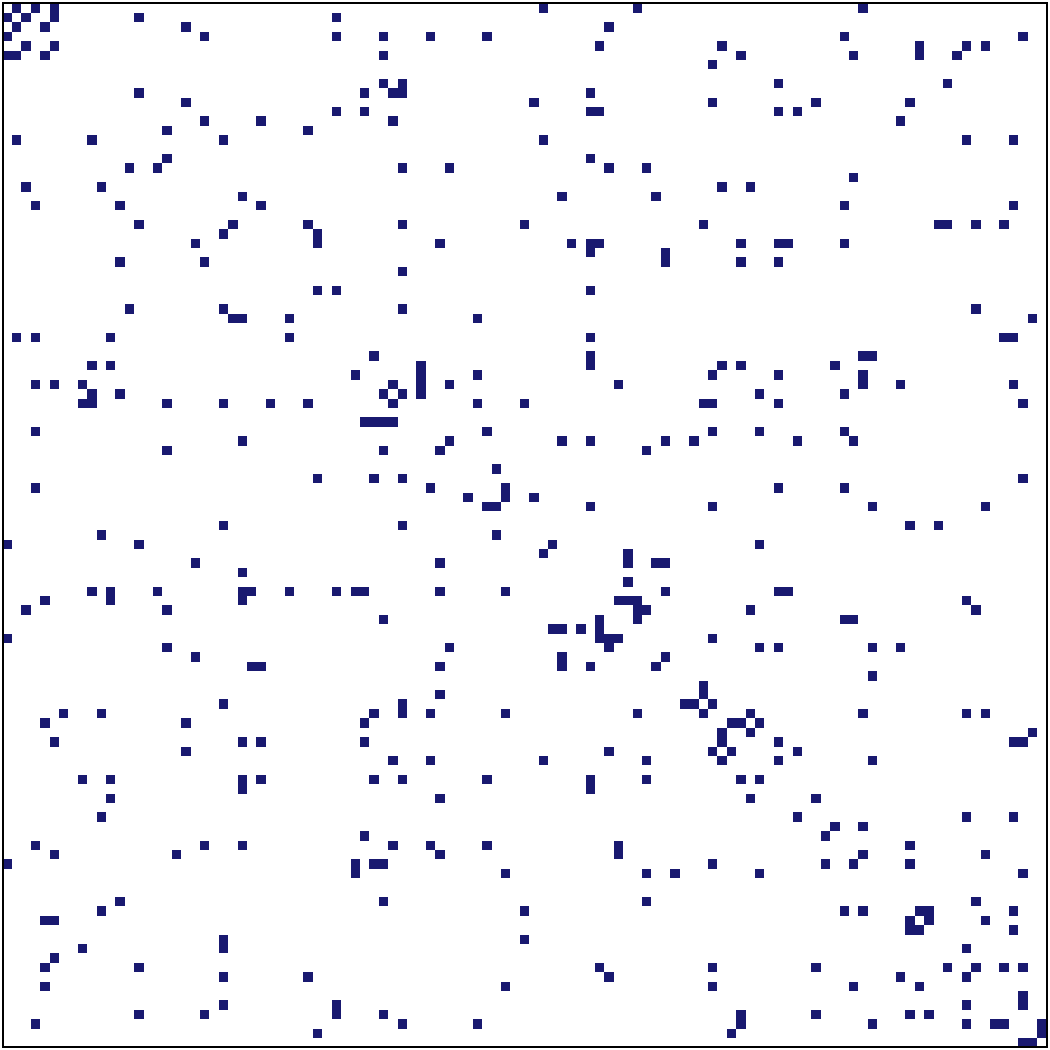
\includegraphics[width=.25\textwidth]{../../chapter/figures/protNet_RATHER}
    & 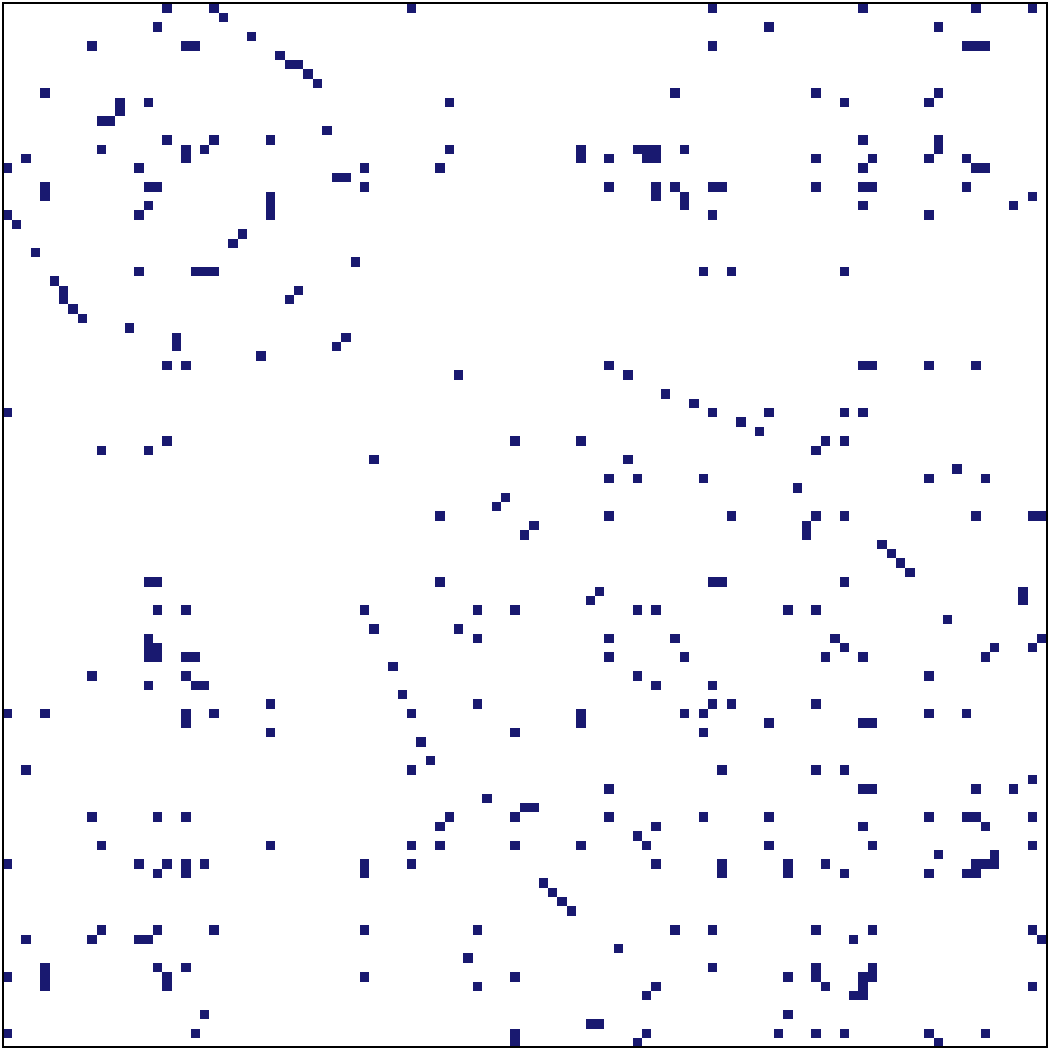
\includegraphics[width=.25\textwidth]{../../chapter/figures/exprNet_RATHER}
    & 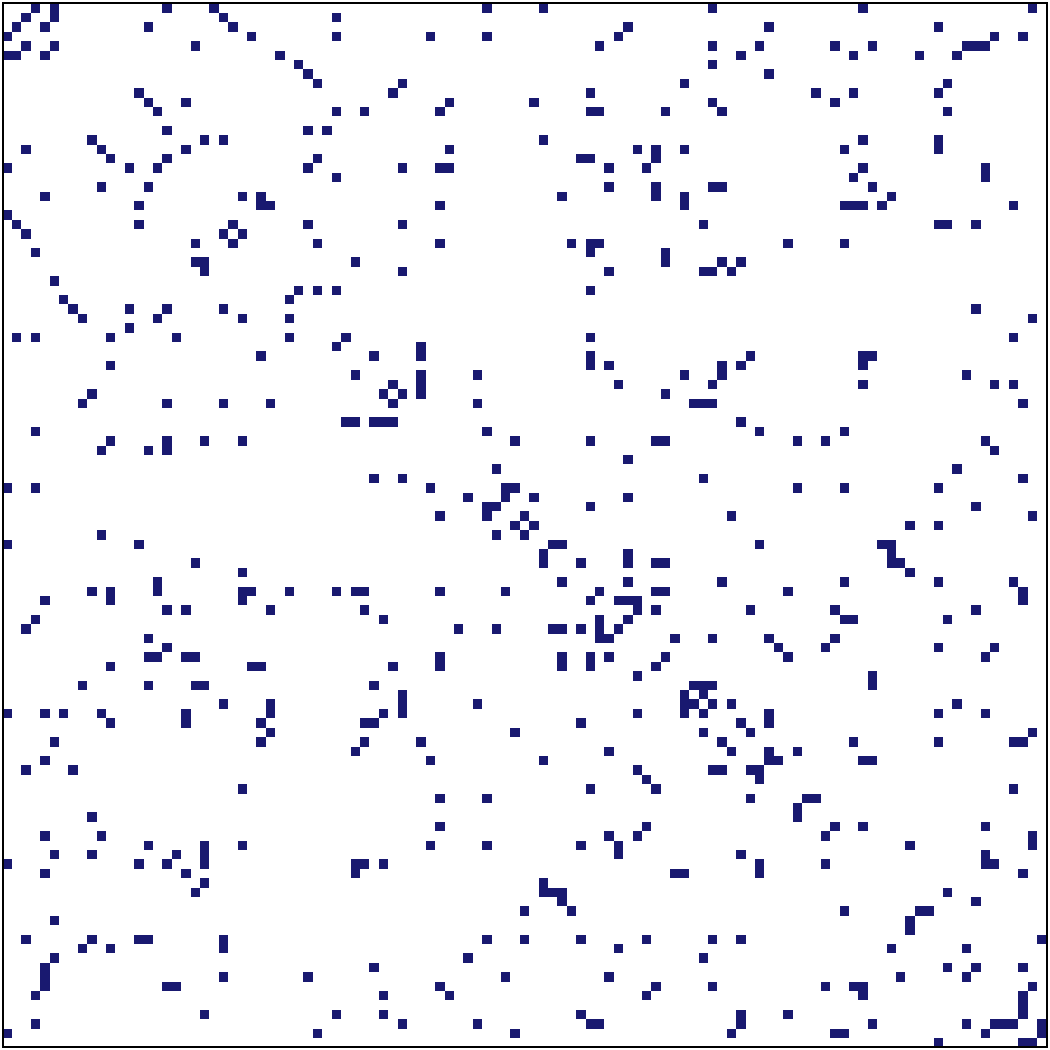
\includegraphics[width=.25\textwidth]{../../chapter/figures/bivarNet_RATHER} \\
  \end{tabular}
  \caption{Uni-attribute and multiattribute networks inferred on both
    NCI60 and RATHER dataset. The number of neighbors of each entity
    is chosen by cross-validation. Multiattribute networks catch motif
    found in the uniattribute counterparts.}
  \label{fig:networks}
\end{figure}

\end{frame}
